\section{Introduction}

In an effort to reduce \gls{tech-debt}, Avigilon is making an effort to
unify code pipelines, compatible with both \gls{gcc} and \gls{msvc}
compilers. New pipelines were developed to take advantage of features
and abilities present in both Linux/\gls{gcc} and Microsoft Windows/\gls{msvc}
based systems, reducing fragmentation between the platforms. Fragmentation of
the codebase increases development time and cost, complexity -- and
therefore the potential for unpredictable or misbehaved functionality -- and
limits extensibility \cite{matjazkljun}. By integrating both platforms with
the same \gls{real-time} processing \gls{pipeline} development time and costs
will be reduced, as well as complexity and the arising potential for
failures or flaws, and increases the ability to and ease of extending and
building on existing functionality. To solve these issues a new \gls{real-time}
processing pipeline was developed, requiring the addition of debugging metrics
to replicate functionality of the old fragmented pipelines and encourage
adoption of the new pipeline by easing debugging.

The implementation of a metrics framework presented many challenges: the
implementation and design of the data collection and processing component (also
referred to as the "metrics unit"), integration of the metrics unit with the new
\gls{pipeline}, and ensuring the solution was cross-platform. The necessity
of cross-platform support was a major factor in the development of the metrics
component as the whole purpose of the development was to reduce codebase fragmentation
between platforms.

Requirements of the metrics component included a \gls{rolling} computation of
a number of metrics: queueing time of the processing pipeline, execution time of
individual \gls{work-unit}, overflow of execution queues, and the servicing
period of each \gls{stream} of different priority. Additionally, the metrics framework
must be lightweight and not interfere with or considerably slow the processing
pipeline. \Gls{threadsafe}ty is another issue which must be considered, as the
metrics component will be interacted with from multiple active pipelines.

By considering these requirements the metrics component and interface to the
existing \gls{pipeline} was designed to provide those benefits of a unified
codebase.

\subsection{The Processing Pipeline}

The \gls{real-time} processing pipeline is utilized when a \gls{stream} requires
processing in real-time, such as a video \gls{stream} from a camera requiring
\glsadd{transcode}transcoding, downsizing, quality reductions, analyzing, or other
manipulations. The processing \gls{pipeline} allows some task to continuously
submit \glspl{work-unit} to be completed, where the data submitted is processed
as a \gls{stream}. The concept of a processing pipeline acting on a stream is
illustrated in Fig.~\ref{fig:pipeline}.

\begin{figure}
	\centering
	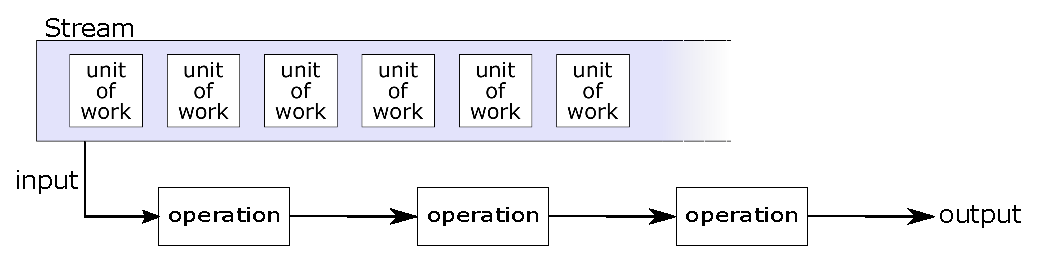
\includegraphics[width=\textwidth]{pipeline}
	\caption{A software pipeline}
	\label{fig:pipeline}
\end{figure}
